% !TeX spellcheck = en_US
\documentclass[french]{yLectureNote}

\title{Outils Mathématiques 2}
\subtitle{Physique}
\author{Paulhenry Saux}
\date{\today}
\yLanguage{Français}

\professor{F.Pettinari}
\usepackage{graphicx}%----pour mettre des images
\usepackage[utf8]{inputenc}%---encodage
\usepackage{geometry}%---pour modifier les tailles et mettre a4paper
%\usepackage{awesomebox}%---pour les boites d'exercices, de pbq et de croquis ---d\'esactiv\'e pour les TP de PC
\usepackage{tikz}%---pour deiffner + d\'ependance de chemfig
% \usepackage{tabularx}%---pour dimensionner automatiquement les tableaux avec variable X
\usepackage{awesomebox}%---Pour les boites info, danger et autres
\usepackage{menukeys}%---Pour deiffner les touches de Calculatrice
\usepackage{fancyhdr}%---pour les en-t\^ete personnalis\'ees
\usepackage{blindtext}%---pour les liens
\usepackage{hyperref}%---pour les liens (\`a mettre en dernier)
\usepackage{caption}%---pour la francisation de la l\'egende table vers Tableau
\usepackage{pifont}
\usepackage{array}%---pour les tableaux
\usepackage{lipsum}
\usepackage{yFlatTable}
\usepackage{multicol}
\newcommand{\Lim}[1]{\lim\limits_{\substack{#1}}\:}
\renewcommand{\vec}{\overrightarrow}
\newcommand{\N}[0]{\mathbb{N}}
\newcommand{\dd}{\mathrm{d}}
\newcommand{\norm}[1]{||\vec{#1}||}
\newcommand{\fo}{\psi(\vec{r},t)}
\newcommand{\foe}{\psi(\vec{r},t)\*}
\newcommand{\HH}{\hat{H}}
\newcommand{\hb}{\hbar}
\newcommand{\lap}{\nabla^2}
\newcommand{\lapcc}{\frac{\partial^2 }{\partial x^2}+\frac{\partial^2 }{\partial y^2}+\frac{\partial^2 }{\partial z^2}}
\newcommand{\mpsi}{\(\psi\)}
\begin{document}
\setcounter{chapter}{1}
\chapter{Règle de Sarrus}

La Règle de Sarrus s'applique uniquement aux matrices carrées d'ordre $3$ ($3 \times 3$). C'est votre outil miracle pour le Jacobien en $\mathbb{R}^3$.

\section{Méthode}
Soit $A$ une matrice $3 \times 3$ :

$$A = \begin{pmatrix}
a & b & c \\
d & e & f \\
g & h & i
\end{pmatrix}$$

La clé est de recopier les deux premières colonnes pour former le schéma d'aide.
\subsection{Étape 1 : Répéter les deux premières colonnes}
$$\begin{pmatrix}
a & b & c \\
d & e & f \\
g & h & i
\end{pmatrix} \begin{array}{cc}
a & b \\
d & e \\
g & h
\end{array}$$
\subsection{Étape 2 : Les Produits positifs}

On somme les produits des éléments situés sur les trois diagonales descendantes (de gauche à droite) :

$$\mathbf{\text{Produits Positifs}} = (\mathbf{\color{checkColor}{a}} \cdot \mathbf{\color{checkColor}{e}} \cdot \mathbf{\color{checkColor}{i}}) + (\mathbf{\color{checkColor}{b}} \cdot \mathbf{\color{checkColor}{f}} \cdot \mathbf{\color{checkColor}{g}}) + (\mathbf{\color{checkColor}{c}} \cdot \mathbf{\color{checkColor}{d}} \cdot \mathbf{\color{checkColor}{h}})$$
\subsection{Étape 3 : Les Produits négatifs}
On soustrait les produits des éléments situés sur les trois diagonales ascendantes (de droite à gauche) :

$$\mathbf{\text{Produits Négatifs}} = (\mathbf{\color{criticalColor}{g}} \cdot \mathbf{\color{criticalColor}{e}} \cdot \mathbf{\color{criticalColor}{c}}) + (\mathbf{\color{criticalColor}{h}} \cdot \mathbf{\color{criticalColor}{f}} \cdot \mathbf{\color{criticalColor}{a}}) + (\mathbf{\color{criticalColor}{i}} \cdot \mathbf{\color{criticalColor}{d}} \cdot \mathbf{\color{criticalColor}{b}})$$
\subsection{Formule complète}

Le déterminant de la matrice $A$ est la somme des produits bleus moins la somme des produits rouges :

$$\det(A) = \underbrace{[(\color{checkColor}{aei}) + (\color{checkColor}{bfg}) + (\color{checkColor}{cdh})]}_{\text{Diagonales descendantes } \searrow} - \underbrace{[(\color{criticalColor}{gec}) + (\color{criticalColor}{hfa}) + (\color{criticalColor}{idb})]}_{\text{Diagonales ascendantes } \nearrow}$$
\subsection{Schéma}
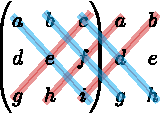
\includegraphics{sarrus.pdf}
 \end{document}
